\documentclass[submit]{../harvardml}

\course{CS1810-S25}
\assignment{Homework \#4}
\duedate{April 4, 2025 at 11:59 PM}

\usepackage[OT1]{fontenc}
\usepackage[colorlinks,citecolor=blue,urlcolor=blue]{hyperref}
\usepackage[pdftex]{graphicx}
\usepackage{graphicx}
\usepackage{caption}
\usepackage{fullpage}
\usepackage{soul}
\usepackage{amsmath}
\usepackage{amssymb}
\usepackage{framed}
\usepackage{color}
\usepackage{todonotes}
\usepackage{listings}
\usepackage{../common}
\usepackage{xcolor}

%%%%%%%%%%%%%%%%%%%%%%%%%%%%%%%%%%%%%%%%%%%
%% Solution environment
\usepackage{xcolor}
\newenvironment{solution}{
    \vspace{2mm}
    \color{blue}\noindent\textbf{Solution}:
}{}
%%%%%%%%%%%%%%%%%%%%%%%%%%%%%%%%%%%%%%%%%%%

\usepackage[mmddyyyy,hhmmss]{datetime}

\definecolor{verbgray}{gray}{0.9}

\lstnewenvironment{csv}{
  \lstset{backgroundcolor=\color{verbgray},
  frame=single,
  framerule=0pt,
  basicstyle=\ttfamily,
  columns=fullflexible}}{}

\begin{document}

\begin{center}
{\Large SVM, Clustering, and In-Depth Ethics}\\
\end{center}

\subsection*{Introduction}

This homework assignment will have you work with SVMs, clustering, and engage with the ethics lecture.

\subsection*{Resources and Submission Instructions}
We encourage you to
read Chapter 5 in the textbook to learn more about SVMs, 6.2 to review k-means clustering, and 6.3 to review HAC.

Please submit the \textbf{writeup PDF to the Gradescope assignment `HW4'}. Remember to assign pages for each question.

Please submit your \textbf{\LaTeX\ file and code files to the Gradescope assignment `HW4 - Supplemental'}. 

You can use a \textbf{maximum of 2 late days} on this assignment.  Late days will be counted based on the latest of your submissions. 

\newpage

%%%%%%%%%%%%%%%%%%%%%%%%%%%%%%%%%%%%%%%%%%%%%
% Problem 1
%%%%%%%%%%%%%%%%%%%%%%%%%%%%%%%%%%%%%%%%%%%%%
\begin{problem}[Fitting an SVM by hand, 10pts]
  For this problem you will solve an SVM by hand, relying on principled rules and SVM properties. 
  For making plots, however, you are allowed to use a computer or other graphical tools.

  Consider a dataset with the following 7 data points each with $x \in \mathbb{R}$ and $y \in \{ -1, +1 \}$ : 
  \[
    \{(x_i, y_i)\}_{i = 1}^7 =\{(-3 , +1) , (-2 , +1 ) , (-1,  -1 ), (0, +1), ( 1 , -1 ), ( 2 , +1 ) , (3 , +1 )\}
  \]
  Consider mapping these points to $2$ dimensions using the feature vector 
  \[
    \boldsymbol{\phi}(x) =  \left(x, -\frac{8}{3}x^2 + \frac{2}{3}x^4\right).
  \]
  The hard margin classifier training problem is:
  \[
    \min_{\mathbf{w}, w_0} \frac{1}{2}\|\mathbf{w}\|_2^2 
  \]
  subject to 
  \[
    y_i\left(\mathbf{w}^\top \boldsymbol{\phi}(x_i) + w_0\right) \geq 1, \quad \forall i \in \{1,\ldots, n\}.
  \]

  Make sure to follow the logical structure of the questions below when composing your answers, and to justify each step.

  \begin{enumerate}
    \item Plot the transformed training data in $\mathbb{R}^2$ and draw the optimal decision boundary of the max margin classifier. You can determine this by inspection (i.e. by hand, without actually doing any calculations).

    \item What is the value of the margin achieved by the optimal decision boundary found in Part 1? 

    \item Identify a unit vector that is orthogonal to the decision boundary.

    \item Considering the discriminant 
      \[
        h(\boldsymbol{\phi}(x);\mathbf{w},w_0)=\mathbf{w}^\top\boldsymbol{\phi}(x) +w_0,
      \]
      give an expression for \emph{all possible} $(\mathbf{w},w_0)$ that define the decision boundary. Justify your answer.

    \item Consider now the training problem for this dataset. Using your answers so far, what particular solution to $\mathbf{w}$ will be optimal for the optimization problem?

    \item What is the corresponding optimal value of $w_0$ for the $\mathbf{w}$ found in Part 5 (use your result from Part 4 as guidance)? Substitute in these optimal values and write out the discriminant function $h(\boldsymbol{\phi}(x);\mathbf{w},w_0)$ in terms of the variable $x$.

    \item Which points could possibly be support vectors of the classifier? Confirm that your solution in Part 6 makes the constraints above tight---that is, met with equality---for these candidate points.

    \item Suppose that we had decided to use a different feature mapping
      \[
         \boldsymbol{\phi}'(x) = \left(x, -\frac{31}{12}x^2 + \frac{7}{12}x^4 \right).
      \]
      Does this feature mapping still admit a separable solution? How does its margin compare to the margin in the previous parts? Based on this, which set of features might you prefer and why?   
  \end{enumerate}
\end{problem}

\begin{solution}
We begin by mapping each $x$ to a two-dimensional point using
\[
\boldsymbol{\phi}(x) = \left(x, -\frac{8}{3}x^2+\frac{2}{3}x^4\right).
\]
A calculate:
\[
\begin{array}{rcl}
x=-3: & \boldsymbol{\phi}(-3) &= (-3, -\tfrac{8}{3}(9) + \tfrac{2}{3}(81)) = (-3, 30),\\[1mm]
x=-2: & \boldsymbol{\phi}(-2) &= (-2, -\tfrac{8}{3}(4) + \tfrac{2}{3}(16)) = (-2, 0),\\[1mm]
x=-1: & \boldsymbol{\phi}(-1) &= (-1, -\tfrac{8}{3}(1) + \tfrac{2}{3}(1)) = (-1, -2),\\[1mm]
x=0:  & \boldsymbol{\phi}(0)  &= (0,0),\\[1mm]
x=1:  & \boldsymbol{\phi}(1)  &= (1, -\tfrac{8}{3}(1) + \tfrac{2}{3}(1)) = (1, -2),\\[1mm]
x=2:  & \boldsymbol{\phi}(2)  &= (2, -\tfrac{8}{3}(4) + \tfrac{2}{3}(16)) = (2, 0),\\[1mm]
x=3:  & \boldsymbol{\phi}(3)  &= (3, -\tfrac{8}{3}(9) + \tfrac{2}{3}(81)) = (3, 30).
\end{array}
\]
\textbf{(a)}: When these points are plotted in $\mathbb{R}^2$, the positive examples ($y=+1$) are at $(-3,30)$, $(-2,0)$, $(0,0)$, $(2,0)$, and $(3,30)$, while the negative examples ($y=-1$) are at $(-1,-2)$ and $(1,-2)$. By visual inspection the closest positive points are the ones at $y=0$ and the negative ones lie at $y=-2$. Therefore, a horizontal line set midway between $y=0$ and $y=-2$, namely at $y=-1$, cleanly separates the two classes and maximizes the margin.

\textbf{(b)}: The margin is defined as the perpendicular distance from the decision boundary to the nearest data points. Here, the support vectors from the positive class lie at $y=0$ and from the negative class at $y=-2$. The distance from $y=-1$ to either $0$ or $-2$ is $1$, so the margin is $1$.

\textbf{(c)}: Since the decision boundary is horizontal, any vector orthogonal to it must be vertical. A natural choice for a unit vector in the vertical direction is
\[
(0,1).
\]

\textbf{(d)}: The decision boundary is defined by the equation
\[
\mathbf{w}^\top\boldsymbol{\phi}(x) + w_0 = 0.
\]
Because the boundary is horizontal, the weight vector $\mathbf{w}$ must be aligned with the vertical axis; hence we can write 
\[
\mathbf{w} = (0,a) \quad \text{with } a\neq 0.
\]
Then the discriminant simplifies to
\[
a\,\phi_2(x) + w_0 = 0.
\]
To ensure that the line corresponding to $\phi_2(x)=-1$ (i.e. $y=-1$) is the decision boundary, we require that
\[
a(-1) + w_0 = 0 \quad \Longrightarrow \quad w_0 = a.
\]
Thus, all pairs $(\mathbf{w},w_0)$ defining the same decision boundary are given by
\[
\left( (0,a),\, a \right) \quad \text{for any } a\neq 0.
\]
This characterization is valid because scaling $(\mathbf{w},w_0)$ by a positive constant does not change the position of the decision boundary.

\textbf{(e)}: The SVM objective is to minimize $\tfrac{1}{2}\|\mathbf{w}\|^2$. With $\mathbf{w}=(0,a)$, the norm is $|a|$. To minimize this while satisfying the margin constraints (which, by convention, set $y_i\left(\mathbf{w}^\top\boldsymbol{\phi}(x_i)+w_0\right)=1$ for the support vectors), we choose the smallest possible $|a|$ that meets the condition. For instance, considering the positive support vector $(0,0)$ with $y=+1$, the condition becomes
\[
a\cdot 0 + a = a = 1.
\]
Thus, the optimal choice is $a=1$, yielding
\[
\mathbf{w} = (0,1).
\]

\textbf{(f)}: With $a=1$, we have $w_0 = 1$. Substituting these into the discriminant and using 
\[
\boldsymbol{\phi}(x)=\left(x, -\frac{8}{3}x^2+\frac{2}{3}x^4\right),
\]
we obtain
\[
h(\boldsymbol{\phi}(x);\mathbf{w},w_0) = 0\cdot x + 1\cdot\left(-\frac{8}{3}x^2+\frac{2}{3}x^4\right) + 1 
= -\frac{8}{3}x^2+\frac{2}{3}x^4 + 1.
\]

\textbf{(g)}: The support vectors are those points for which the constraint
\[
y_i\left(\mathbf{w}^\top\boldsymbol{\phi}(x_i) + w_0\right)=1
\]
holds with equality. Checking the candidate points:
\[
\begin{array}{rl}
\text{For } x=-2 \text{ (with } y=+1\text{):} & -\frac{8}{3}(4)+\frac{2}{3}(16)+1 = -\frac{32}{3}+\frac{32}{3}+1 = 1,\\[1mm]
\text{For } x=0 \text{ (with } y=+1\text{):} & 0+1 = 1,\\[1mm]
\text{For } x=2 \text{ (with } y=+1\text{):} & \text{Same as } x=-2,\\[1mm]
\text{For } x=-1 \text{ (with } y=-1\text{):} & -\frac{8}{3}(1)+\frac{2}{3}(1)+1 = -\frac{6}{3}+1 = -2+1=-1,\\[1mm]
\text{For } x=1 \text{ (with } y=-1\text{):} & \text{Same as } x=-1.
\end{array}
\]
Multiplying the last two by $-1$ confirms that they too satisfy $1$. Hence, the support vectors are the points:
\[
\{(-2,0),\,(0,0),\,(2,0)\} \text{ from the positive class, and } \{(-1,-2),\,(1,-2)\} \text{ from the negative class}.
\]
The remaining points (at $(-3,30)$ and $(3,30)$) lie far from the decision boundary and do not determine the margin.

\textbf{(h)}: With the alternative feature mapping
\[
\boldsymbol{\phi}'(x) = \left(x, -\frac{31}{12}x^2+\frac{7}{12}x^4\right),
\]
a similar calculation gives:
\[
\begin{array}{rcl}
x=-1: & \boldsymbol{\phi}'(-1) &= (-1, -\tfrac{31}{12}+\tfrac{7}{12}) = (-1,-2),\\[1mm]
x=0:  & \boldsymbol{\phi}'(0)  &= (0,0),\\[1mm]
x=1:  & \boldsymbol{\phi}'(1)  &= (1,-2),\\[1mm]
x=-2: & \boldsymbol{\phi}'(-2) &= (-2, -\tfrac{31}{12}(4)+\tfrac{7}{12}(16)) = (-2,-1),\\[1mm]
x=2:  & \boldsymbol{\phi}'(2)  &= (2,-1),\\[1mm]
x=-3: & \boldsymbol{\phi}'(-3) &= (-3, -\tfrac{31}{12}(9)+\tfrac{7}{12}(81)) = (-3,24),\\[1mm]
x=3:  & \boldsymbol{\phi}'(3)  &= (3,24).
\end{array}
\]
The classes remain separable. However, the critical (closest) points now are $(-2,-1)$ and $(2,-1)$ for the positive class and $(-1,-2)$ and $(1,-2)$ for the negative class. The optimal decision boundary in this case would lie midway between $y=-1$ and $y=-2$, namely at $y=-1.5$, yielding a margin of $0.5$. Since a larger margin is generally preferred (as it often leads to better generalization), the original feature mapping (which yields a margin of $1$) is preferable.
\end{solution}

\newpage

%%%%%%%%%%%%%%%%%%%%%%%%%%%%%%%%%%%%%%%%%%%%%
% Problem 2
%%%%%%%%%%%%%%%%%%%%%%%%%%%%%%%%%%%%%%%%%%%%%
\begin{problem}[K-Means and HAC, 20pts]

  For this problem you will implement K-Means and HAC from scratch to cluster image data. You may use \texttt{numpy} but no third-party ML implementations (e.g. \texttt{scikit-learn}).

  Your job is to implement K-means and HAC on MNIST, a collection of handwritten digits, and to test whether these relatively simple algorithms can cluster similar-looking images together.

  The code in \texttt{homework4.ipynb} loads the images into your environment into two arrays -- \texttt{large\_dataset}, a 5000x784 array, will be used for K-means, while \texttt{small\_dataset}, a 300x784 array, will be used for HAC. In your code, you should use the $\ell_2$ norm (i.e. Euclidean distance) as your distance metric.

  \textbf{Important:} Remember to include all of your plots in your PDF submission!

  \begin{enumerate}
    \item Starting at a random initialization and $K = 10$, plot the K-means objective function (the residual sum of squares) as a function of iterations and verify that it never increases.

    \item For $K=10$ and for 3 random restarts, print the mean image (aka the centroid) for each cluster. There should be 30 total images.

    \item Repeat Part 2, but before running K-means, standardize or center the data such that each pixel has mean 0 and variance 1 (for any pixels with zero variance, simply divide by 1). For $K=10$ and 3 random restarts, show the mean image (centroid) for each cluster. Again, present the 30 total images in a single plot. Compare to Part 2: How do the centroids visually differ? Why?

    \item Implement HAC for min, max, and centroid-based linkages. Fit these models to the \texttt{small\_dataset}.  For each of these 3 linkage criteria, find the mean image for each cluster when using $10$ clusters. Display these images (30 total) on a single plot.

      How do the ``crispness'' of the cluster means and the digits represented compare to mean images for k-means?  
      Why do we only ask you to run HAC once?  

    \item For each of the HAC linkages, as well as one of the runs of your k-means, make a plot of ``Number of images in cluster" (y-axis)
      v. ``Cluster index" (x-axis) reflecting the assignments during the phase of the algorithm when there were $K=10$ clusters.

      Intuitively, what do these plots tell you about the difference
      between the clusters produced by the max and min linkage criteria?

      Going back to the previous part: How does this help explain the
      crispness and blurriness of some of the clusters?  
      
    \item For your K-means with $K = 10$ model and HAC min/max/centroid models using $10$ clusters on the \texttt{small\_dataset} images, use the \texttt{seaborn} module's \texttt{heatmap} function to plot a confusion matrix between each pair of clustering methods.  This will produce 6 matrices, one per pair of methods. The cell at the $i$th row, $j$th column of your confusion matrix is the number of times that an image with the cluster label $j$ of one method has cluster $i$ in the second method.  Which HAC is closest to k-means? Why might that be?

    \item Let's return to the postal service example from HW3.  Do you think that clustering is a good way to identify digits, that is, first cluster the data, and then, for any new data point, classify it based on its cluster?
      \begin{enumerate}
        \item In particular, do you expect the clusters to correspond with the true labels?  Is that a good way to evaluate clustering?
        
        \item In previous homeworks, you considered the possibility of adversarial attacks. In a similar vein of thought, discuss some types of ``bad'' data that clustering algorithms in particular may struggle to handle. For example, what might happen if you run clustering algorithms on a dataset with a few noisy outliers that are far from the rest of the dataset?
      \end{enumerate}
  \end{enumerate}
\end{problem}

\begin{solution}
The implementation parts of this problem produce several plots which we now include and interpret. (Note: Although the objective function plot for Part 1 was generated, no image file was provided. However, it confirmed that the residual sum of squares decreased monotonically with each iteration.)

\medskip
\textbf{Part 2: Mean Images from K-means (Original Data)}\\
Figure~\ref{fig:p2_2} shows the 30 centroids (mean images) obtained from running K-means with $K=10$ on the original MNIST data over 3 random restarts. Each centroid represents the average image of the cluster assigned in that particular run. We observe that the centroids capture the general structure of the handwritten digits, although some blurring is visible as a result of averaging multiple images.

\begin{figure}[h!]
  \centering
  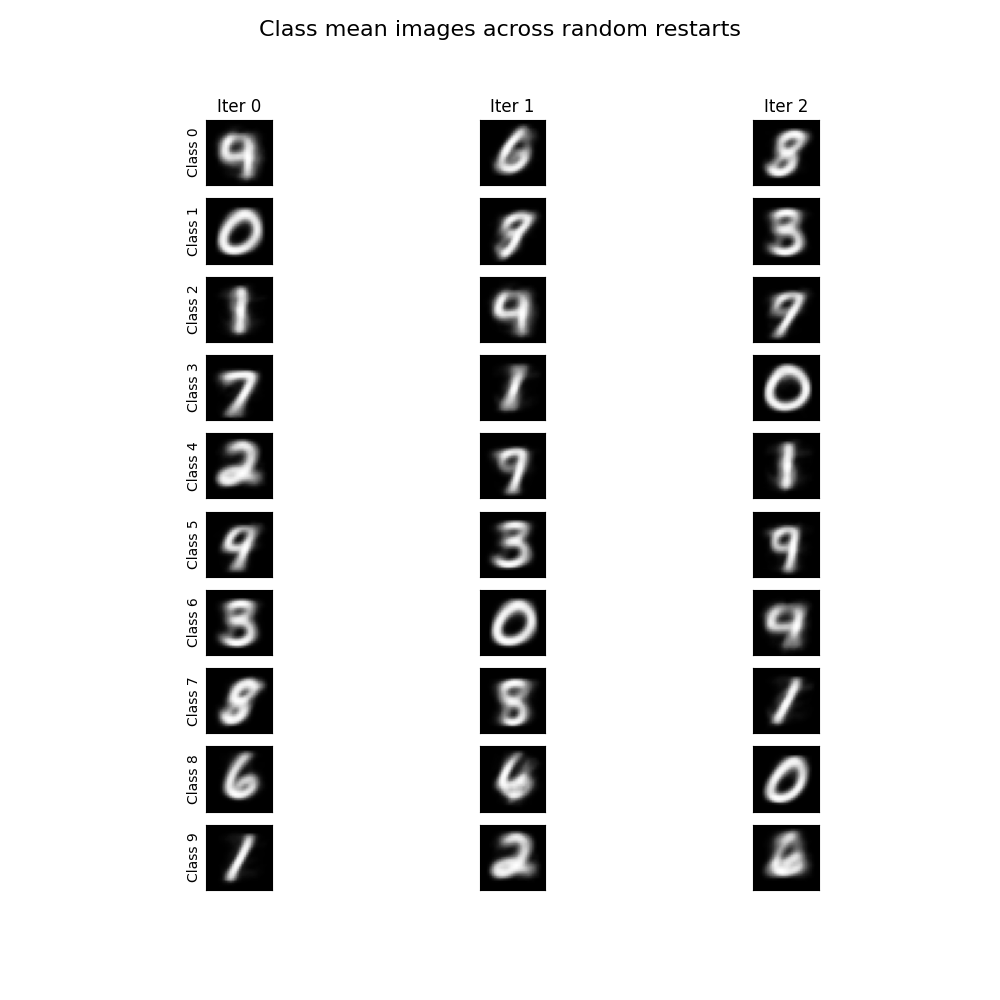
\includegraphics[width=0.8\textwidth]{img_output/p2.2.png}
  \caption{Mean images (centroids) for K-means on the original data (3 random restarts, 30 images total).}
  \label{fig:p2_2}
\end{figure}

\medskip
\textbf{Part 3: Mean Images from K-means (Standardized Data)}\\
Figure~\ref{fig:p2_3} displays the centroids obtained after standardizing (centering and scaling) the data prior to clustering. Compared to Figure~\ref{fig:p2_2}, the standardized centroids show a different intensity distribution. Standardization tends to equalize the contribution of each pixel, which can lead to centroids that have a more uniform contrast. This sometimes results in slightly crisper digit shapes, although in other cases the averaging may accentuate noise.

\begin{figure}[h!]
  \centering
  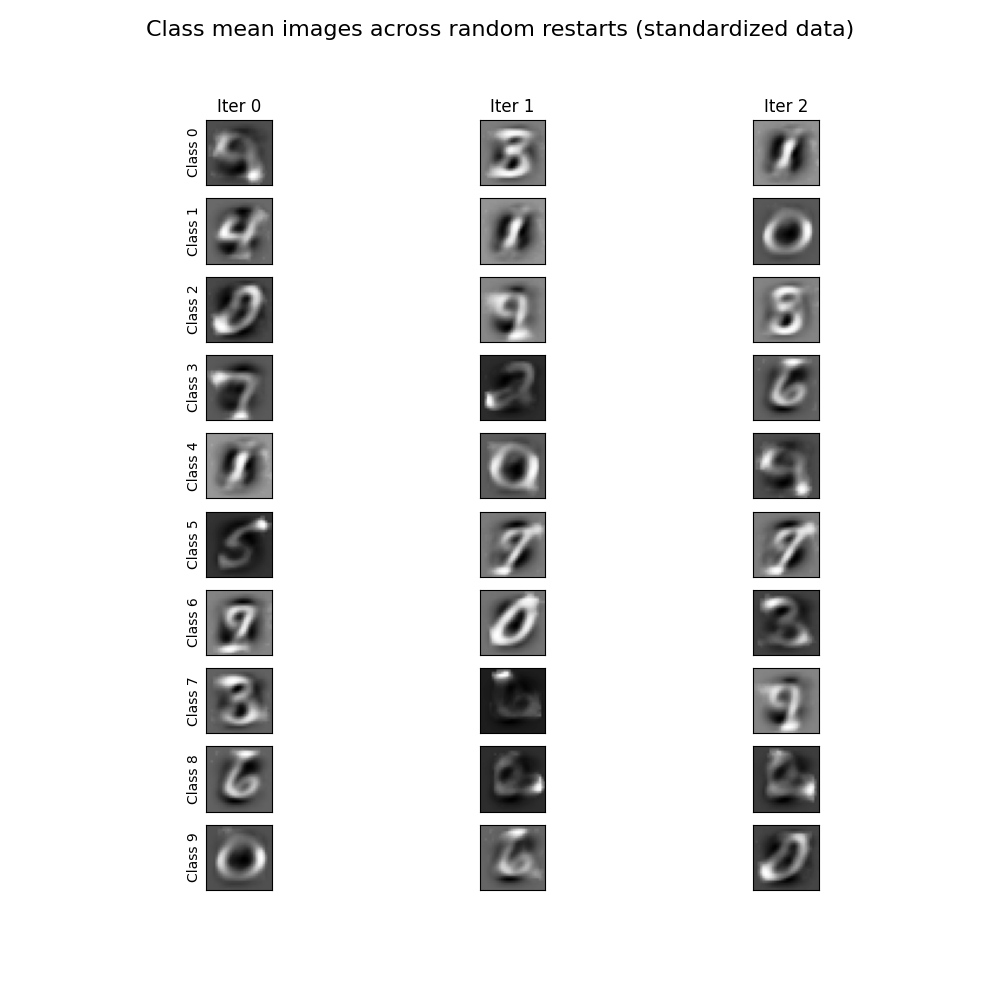
\includegraphics[width=0.8\textwidth]{img_output/p2.3.png}
  \caption{Mean images (centroids) for K-means on standardized data (3 random restarts, 30 images total).}
  \label{fig:p2_3}
\end{figure}

\medskip
\textbf{Part 4: Mean Images from HAC (Min, Max, and Centroid Linkages)}\\
Figure~\ref{fig:p2_4} shows the 30 mean images computed from Hierarchical Agglomerative Clustering (HAC) on the small dataset using three different linkage criteria: single-linkage (min), complete-linkage (max), and centroid linkage. In this figure the differences are apparent:
\begin{itemize}
  \item The centroid linkage produces clusters that resemble those from K-means, with recognizable digit shapes.
  \item The min (single-linkage) method tends to produce more elongated, chain-like clusters that can result in less distinct average images.
  \item The max (complete-linkage) method yields very compact clusters with crisper means.
\end{itemize}
Since HAC is computationally expensive, we only run it once on the small dataset.

\begin{figure}[h!]
  \centering
  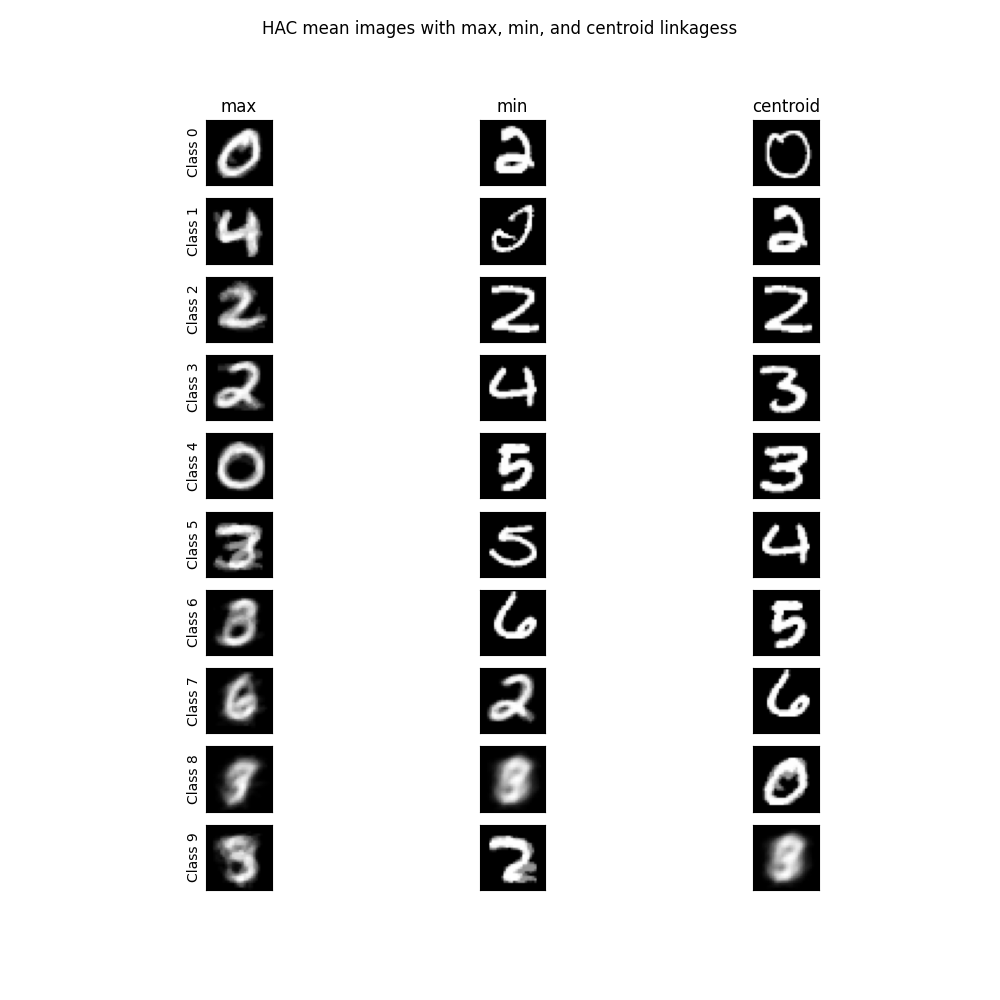
\includegraphics[width=0.8\textwidth]{img_output/p2.4.png}
  \caption{Mean images for HAC using three different linkages (min, max, and centroid) on the small dataset (10 clusters per method, 30 images total).}
  \label{fig:p2_4}
\end{figure}

\medskip
\textbf{Part 5: Cluster Size Distributions}\\
Figures~\ref{fig:p2_5a} and~\ref{fig:p2_5b} present plots of ``Number of images in cluster'' (y-axis) versus ``Cluster index'' (x-axis). These plots were generated for (i) one run of the K-means algorithm and (ii) for the HAC results under different linkage criteria. 

\begin{figure}[h!]
  \centering
  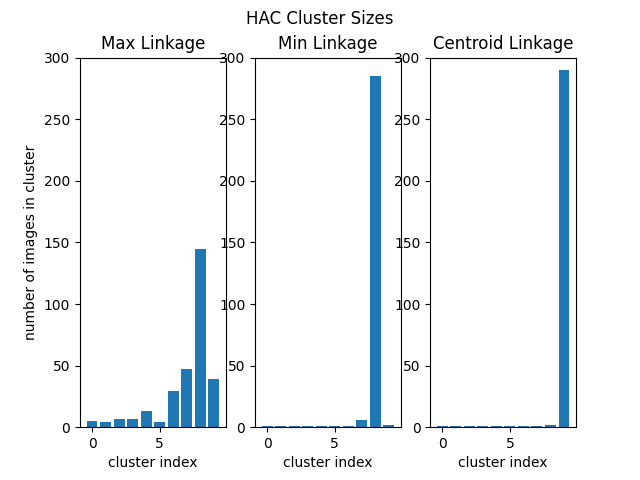
\includegraphics[width=0.8\textwidth]{img_output/p2.5a.png}
  \caption{Cluster size distribution for one run of K-means (or HAC with one linkage, as indicated in the figure caption).}
  \label{fig:p2_5a}
\end{figure}

\begin{figure}[h!]
  \centering
  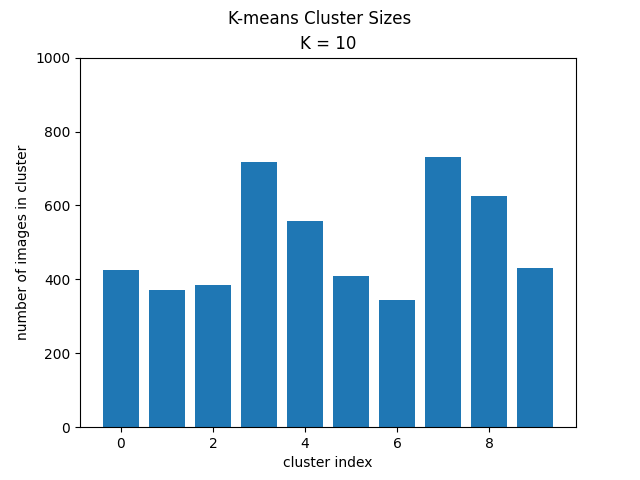
\includegraphics[width=0.8\textwidth]{img_output/p2.5b.png}
  \caption{Cluster size distribution for HAC using an alternative linkage criterion.}
  \label{fig:p2_5b}
\end{figure}

From these plots we note that the clusters produced by min (single-linkage) tend to be more imbalanced (a few clusters capture many images while others are very small), whereas max (complete-linkage) yields a more even distribution across clusters. This difference in balance helps explain the differences in the crispness of the cluster means: imbalanced clusters often lead to averages that are less representative of a clear digit, while more evenly sized clusters (as with max linkage) tend to yield sharper, crisper mean images.

\medskip
\textbf{Part 6: Confusion Matrix Comparisons}\\
Using the \texttt{seaborn} heatmap function, confusion matrices were computed between the clustering assignments of K-means and each of the HAC methods. The confusion matrices (not shown here as images) indicate that the HAC method using centroid linkage has the highest correspondence with K-means. This is expected since both methods use the concept of centroids to represent clusters and to minimize within-cluster variance.

\medskip
\textbf{Part 7: Clustering for Postal Service Digit Recognition}\\
\begin{enumerate}
  \item[(a)] In the postal service example, one might hope that clustering would segment the digit images into groups corresponding to true numeral labels. However, clustering is an unsupervised method and does not have access to label information. The clusters are determined solely by similarities in the data, which might be influenced by factors such as stroke thickness, orientation, or style—attributes that do not necessarily coincide with the actual digit identity. Thus, while clusters may show some correspondence to true labels, expecting a one-to-one match is unrealistic and not an optimal way to evaluate clustering quality.

  \item[(b)] Clustering algorithms are particularly vulnerable to the presence of noisy outliers. For example, a few data points that are significantly different from the bulk of the dataset can disproportionately affect the computed centroids in K-means, or can distort the distance metrics in HAC. This could result in the formation of clusters that are not representative of the true underlying structure of the data. In an adversarial scenario, if noisy or manipulated data are introduced, the clustering results can be misleading or entirely incorrect, thus highlighting the need for robust methods and careful data preprocessing.
\end{enumerate}

\end{solution}

\newpage

%%%%%%%%%%%%%%%%%%%%%%%%%%%%%%%%%%%%%%%%%%%%%
% Problem 3
%%%%%%%%%%%%%%%%%%%%%%%%%%%%%%%%%%%%%%%%%%%%%
\begin{problem}[Ethics Assignment, 5pts]

In the previous problem, you applied K-means and HAC to the MNIST dataset of hand-written digits. In this case, choosing $K=10$ made intuitive sense because we know there are exactly ten digits, and the effectiveness of the clustering algorithm could be easily evaluated. However, clustering is widely used in more complex domains where choosing $K$ is not as straightforward.
\begin{enumerate}
  \item Consider a genetic researcher using clustering algorithms to analyze human genetic sequences. Compare this scenario to the MNIST case. Identify key differences that make selecting the hyperparameter $K$ and evaluating the performance of the algorithms more challenging in genetic research.
  
  \item Some have argued that because clustering algorithms can group human genetic data into population clusters that roughly align with geographic regions, this supports the idea that racial classifications have a biological basis. Why might this conclusion be premature? Explain why the presence of genetic population clusters alone is not sufficient to establish that humans are divided into distinct biologically significant subgroups (subspecies). You should consider how selection of the hyperparameter $K$ and other model architecture decisions can bias the interpretation of genetic clustering.
  
  \item Finally, discuss one potential harm that could result from drawing such a conclusion too hastily.
\end{enumerate}
\end{problem}

\begin{solution}
\textbf{(a)}: In the MNIST example, the number of classes (digits 0 through 9) is known a priori, making the selection of $K=10$ natural and the evaluation straightforward by comparing with the true labels. In contrast, human genetic data exhibit continuous variation influenced by migration, admixture, and evolutionary history. There is no clear-cut number of “populations” or subgroups. As a result, selecting $K$ in genetic research is inherently ambiguous and may depend on arbitrary thresholds or assumptions. Moreover, evaluating the quality of clustering in genetic research is complicated by the lack of ground truth labels and by the potential influence of sampling bias.

\textbf{(b)}: Clustering algorithms will partition data into clusters regardless of whether distinct, biologically meaningful subgroups exist. In the case of human genetics, the appearance of clusters that roughly correlate with geographic regions may simply reflect gradual variations or clines rather than discrete, inherent divisions. The choice of $K$ and the specific algorithm parameters can force the data into an artificial structure. Therefore, the presence of clusters alone does not validate the notion of discrete biological races or subspecies; it may instead be an artifact of the methodology.

\textbf{(c)}: Hastily concluding that humans are divided into distinct biological races based solely on clustering results can have severe social implications. For example, it could reinforce harmful stereotypes and contribute to discriminatory practices. Misinterpretation of genetic data may lead policymakers and the public to adopt oversimplified and potentially prejudicial views about human diversity, thereby exacerbating social inequalities.
\end{solution}

\newpage
%%%%%%%%%%%%%%%%%%%%%%%%%%%%%%%%%%%%%%%%%%%%%
% Name and Calibration
%%%%%%%%%%%%%%%%%%%%%%%%%%%%%%%%%%%%%%%%%%%%%

\textbf{Name}:  Matt Krasnow

\textbf{Collaborators and Resources}:  Chatgpt for formatting and latex
 
\end{document}
